

\documentclass{beamer}
\usetheme{metropolis}

\usepackage{tcolorbox}

\usepackage[utf8]{inputenc} % allow utf-8 input
\usepackage[T1]{fontenc}    % use 8-bit T1 fonts
\usepackage{hyperref}       % hyperlinks
\usepackage{url}            % simple URL typesetting
\usepackage{booktabs}       % professional-quality tables
\usepackage{amsfonts}       % blackboard math symbols
\usepackage{nicefrac}       % compact symbols for 1/2, etc.
\usepackage{microtype}      % microtypography
\usepackage{xcolor}         % colors
\usepackage{graphicx}
\usepackage{float}
\usepackage{amsmath}
\tcbuselibrary{skins}

\newtcolorbox{mybubble}[1][]{
  enhanced jigsaw,
  borderline={1pt}{-2pt}{gray, sharp corners},
  frame hidden,
  left=1mm,
  right=1mm,
  fontupper=\scriptsize,
  arc=1mm,
  #1
}


\title{Exploring Data Cleaning using Language Model for Sentiment Classification Task}
\author{Puttisan "Ninja" Mukneam}
\institute{Pitzer College}
\date{\today}

% Customize footline
\setbeamertemplate{footline}
{
  \leavevmode%
  \hbox{%
  \begin{beamercolorbox}[wd=.25\paperwidth,ht=2.25ex,dp=1ex,center]{author in head/foot}%
    \usebeamerfont{author in head/foot}\insertauthor
  \end{beamercolorbox}%
  \begin{beamercolorbox}[wd=.75\paperwidth,ht=2.25ex,dp=1ex,center]{title in head/foot}%
  \end{beamercolorbox}}%
  \vskip0pt%
}

\begin{document}

\begin{frame}
\titlepage
\end{frame}

\begin{frame}
\frametitle{Overview of Data Cleaning for Machine/Deep Learning}

\begin{itemize}
\item \textbf{Data cleaning:} The process of identifying and correcting or removing errors, inconsistencies, and inaccuracies in datasets to improve data quality and ensure reliable results.
\item \textbf{Importance:} High-quality data is crucial for training effective machine learning and deep learning models, as it directly impacts their performance and generalization abilities.
\item \textbf{Common issues:}
\begin{itemize}
\item Missing values
\item Duplicate records
\item Inconsistent formats
\item Incorrect data types
\item Outliers and anomalies
\end{itemize}
\end{itemize}

\end{frame}

\begin{frame}{Overview: Continue}
\begin{itemize}

\item \textbf{Traditional cleaning techniques:}
\begin{itemize}
\item Imputation
\item Deduplication
\item Standardization
\item Data transformation
\item Outlier detection and removal
\end{itemize}

\item \textbf{Why do we want to clean data in Sentiment Task ?}

\begin{itemize}
    \item Noise Reduction
    \item Standardization
    \item Reducing Dimensionality
    \item Handling Missing/Incomplete Data
    \item Improve model performance
\end{itemize}

    \end{itemize}



\end{frame}

\begin{frame}
\frametitle{Literature Review: CleanML}

\begin{itemize}
\item \textbf{Reference:} CleanML: A Study for Evaluating the Impact of Data Cleaning on ML Classification Task, by Peng Li, others (2021).

\item \textbf{Robust algorithms:} Researchers have attempted to develop robust machine/deep learning algorithms that can handle dirty/noisy data without the need for data cleaning.

\item \textbf{Drawbacks of robust algorithms:}
\begin{itemize}
\item Limited generalization capabilities: Robust algorithms might perform well on specific types of noisy data but fail to generalize to other types or levels of noise.

\item Overfitting: These algorithms may overfit the training data, leading to poor performance on unseen data.

\item Increased complexity: Designing and implementing robust algorithms can be more complex and computationally expensive.
\end{itemize}

\end{itemize}

\end{frame}

\begin{frame}{CleanML: Continue}
\begin{itemize}
    \item \textbf{CleanML findings:} The study reveals that cleaning data before training tend to improve the performance of machine learning classifiers.
\begin{itemize}
\item Higher accuracy when filling out Missing Values, cleaning outliers, cleaning mislabels, cleaning mislabels, but insignificant or even negative impact on cleaning duplicates.

\item Better generalization: Models trained on cleaned data are more likely to generalize well to new, unseen data, and can be used with many ML/DL algorithms

\end{itemize}
\end{itemize}
    
\end{frame}

\begin{frame}
  \frametitle{Justifying Transformers and Language Models for Data Cleaning}

  \begin{itemize}
    \item \textbf{Context-awareness:} Transformers and language models like ChatGPT and T5 have a deep understanding of natural language and can efficiently handle context in textual data.

    \item \textbf{Semantic understanding:} These models can accurately identify and remove non-sentimental words from a review, preserving only the words that contribute to the overall sentiment.

  \end{itemize}

\end{frame}

\begin{frame}{Justification: Continue}
\begin{itemize}
\item \textbf{Scalability:} Language models, when properly trained and fine-tuned, can handle data of any size and perform data cleaning tasks effectively and efficiently. This can help to scale data cleaning techniques for large and rapidly growing datasets in the Big Data era.
    
    \item \textbf{User Engagement:} With an optimized language model, the need for human intervention in data cleaning tasks can be significantly reduced. This not only increases the efficiency of the process but also mitigates the risks of human errors.
    
    \item \textbf{Semi-structured and unstructured data:} The use of machine learning tools can help detect the type of data and structure it appropriately before passing it into the cleaning model. This can help address data quality problems for semi-structured and unstructured data formats.
    
 
\end{itemize}
    
\end{frame}

\begin{frame}{Justification: Continue}

\begin{itemize}
    
    \item \textbf{Privacy and Security Concerns:} Due to the automated nature of the data cleaning process using language models, human intervention is minimized, thereby addressing privacy and security concerns. An optimized language model doesn't require access to raw data, which can help to ensure privacy.

\end{itemize}
\end{frame}

\section{Language  Model}

\begin{frame}{Language Model}

Language models are designed to understand and generate human-like text based on the input they receive. These models use deep learning techniques, particularly variants of the Transformer architecture, to process and generate text.

Once the model has processed the input, it generates a response by predicting the most probable sequence of words or tokens based on its training. It considers the context of the input, including the prompt and any previous conversation history, to produce a coherent and relevant output.
\end{frame}

\begin{frame}{Language Model}

$$P_\theta (X_{t+1} = x_{t+1} | x_1, \cdots, x_t)$$

Predicting next words given its history (previous words). And try to find $\theta$ (parameter of the model) that maximize above probability
\end{frame}



\begin{frame}{Example}
History:

I love ?

Next words:

\begin{align*}
    P_\theta(? = this | history) = 0.4\\
    P_\theta(? = game | history) = 0.3\\
    P_\theta(? = buy | history) = 0.04\\
    \vdots
\end{align*}

\end{frame}

\begin{frame}{Models}

\begin{table}[h]
\centering
\begin{tabular}{ll}
\toprule
\textbf{Model} & \textbf{Number of Parameters} \\
\midrule
gpt2 & 117M\\
gpt2-xl & 1558M\\
t5-base & 250M\\
t5-xl & 3000M\\
flan-t5-base & 250M\\
flan-t5-xl & 3000M \\
\bottomrule
\end{tabular}
\caption{Pre-tranied models}
\end{table}
    
\end{frame}




\begin{frame}{Transformer: }
\textbf{Motivation}
\begin{itemize}
    \item Limit lengths of signal paths required to learn long-range dependencies
    \item  parallelization in training phase 
\end{itemize}
\textbf{Overview}
\begin{itemize}
    \item multi-layer of "attention" generating new representation of given tokens to account for context of the whole text.
\end{itemize}
\end{frame}

\begin{frame}{Addressing RNN}
        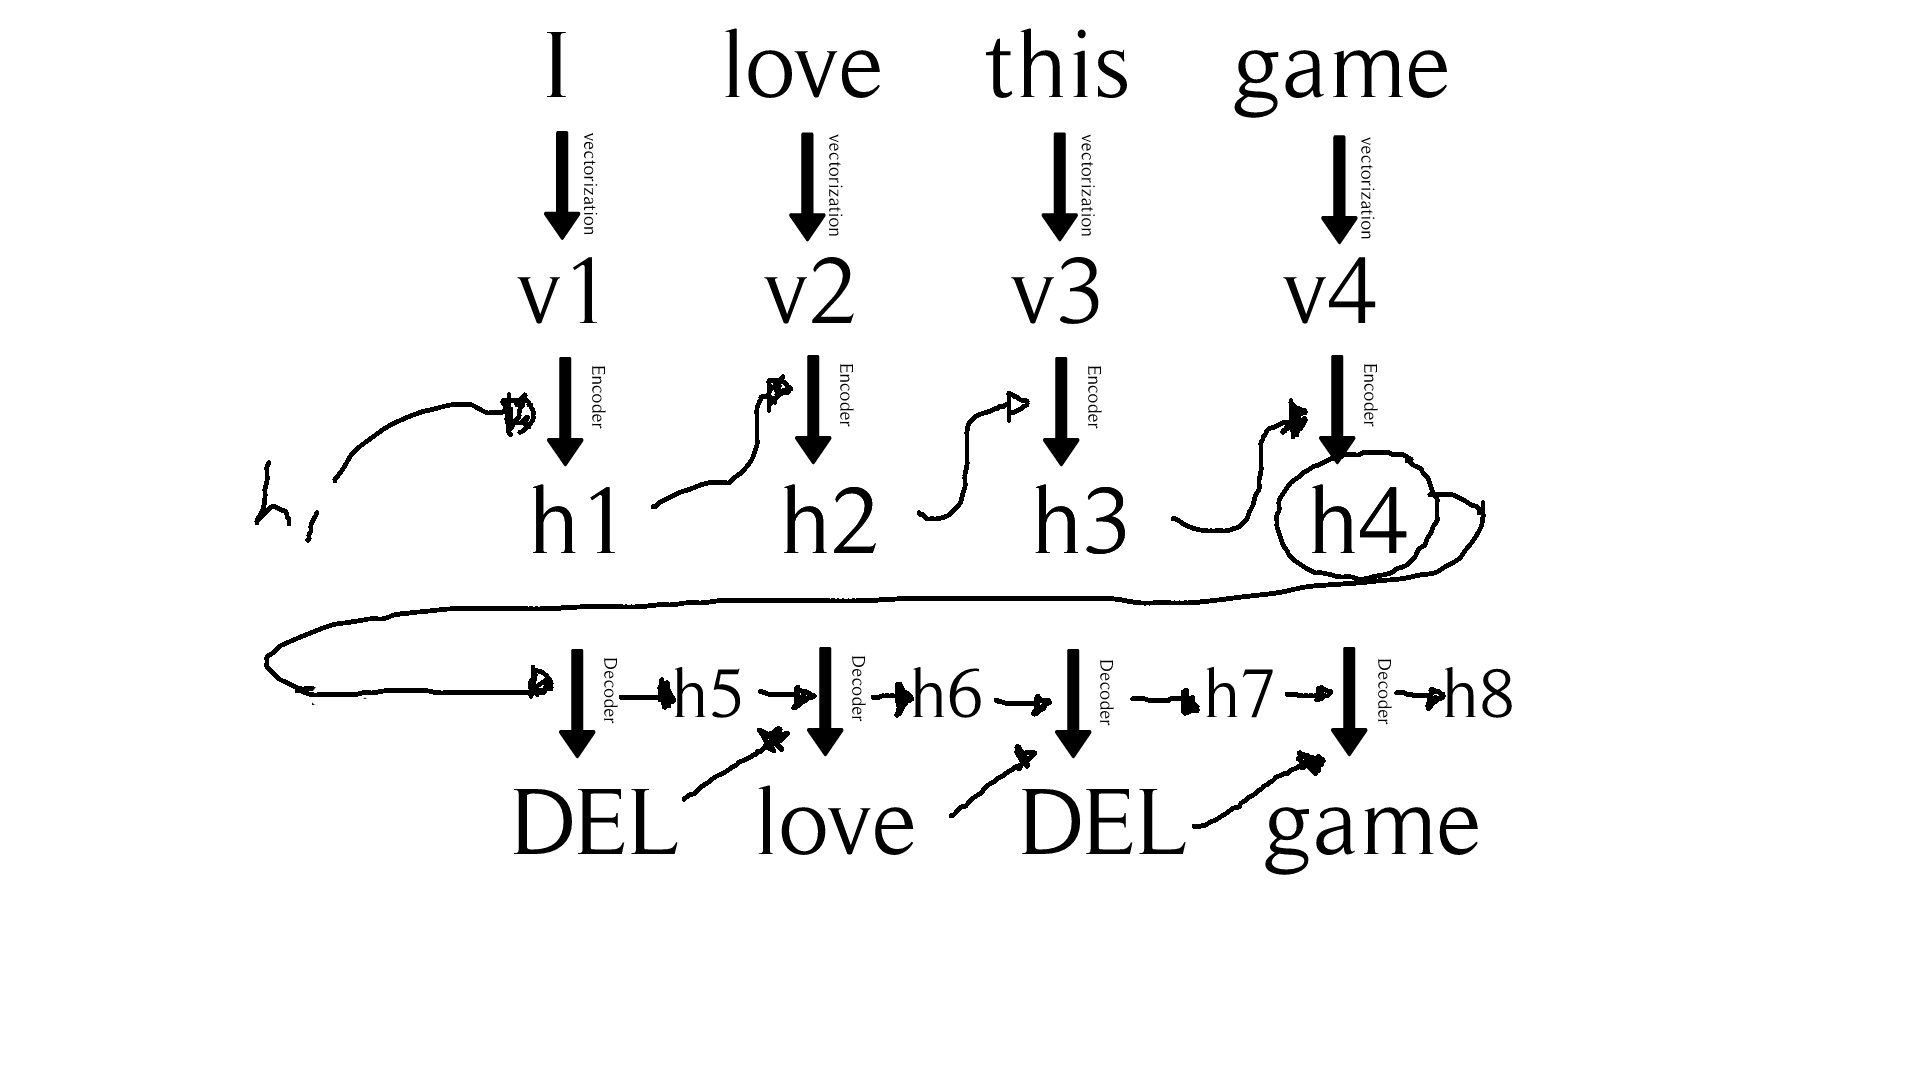
\includegraphics[scale=0.2]
{img/RNN_sim.jpg}
\centering
\end{frame}

\begin{frame}{Transformer's model architecture}
    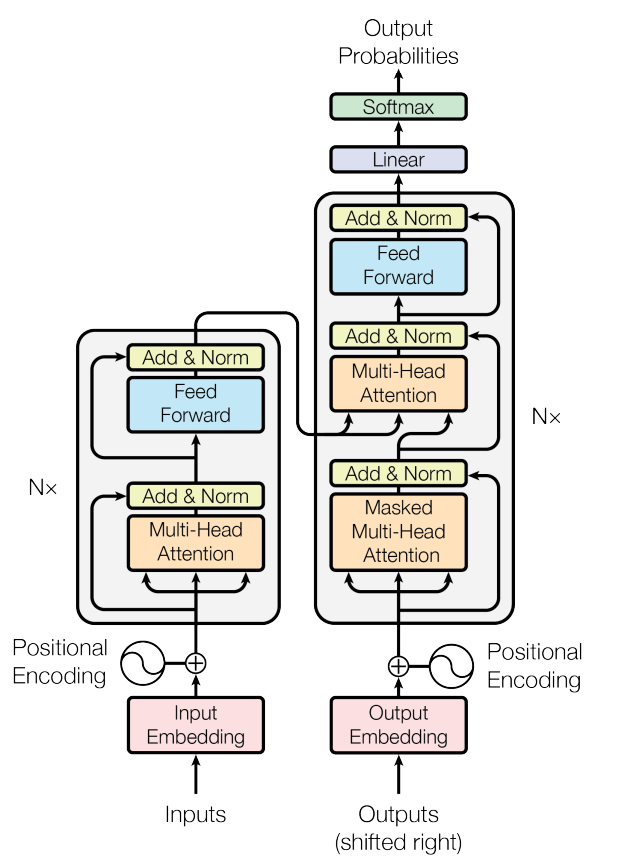
\includegraphics[scale=0.35]
{img/trans_arch.png}
\centering
\end{frame}

\begin{frame}{GPT-3: Overview}
\begin{itemize}
    \item modified transformer to be LLM
    \item 175 Billion parameters with 96 Layers of NN
    \item unsupervised trained on 500 Billion tokens ("Common Crawl", i.e., all most every (improved) text on the internet + books + wikipedia)
    \item Goal: given a text, generate the response
    \item Was supervised fine-tune for safety (Reinforcement Learning) using PPO (iterative-improvment) and reward system (from user's feedback)
\end{itemize}

\end{frame}

\begin{frame}{GPT-3: Training}
\begin{itemize}
    \item Proposed to just pre-train, then add example, then perform the task. (one-shot, few-shot) i.e., no fine-tuning
\end{itemize}
    
\end{frame}

\begin{frame}{High-Level Procedure}
\textbf{Template} := \textit{Task Description}:\textit{prompt} \\
\textbf{Example}: Without explaining, keep only words that imply sentiment of the author in an array: "I love this game"
\begin{itemize}
    \item  Tokenization/Embedding $\Rightarrow$ [3, 200, 150, 60, ...] 
    \item Gathering "example", i.e., previous response, etc.
    \item Processing Layers through self-attention outputting new representation that captures the context in the given text
    \item Output generation by looking at the probability distribution for the next token
    \item  Decode  $\Rightarrow$ ['love', 'game']
    \item Post-processing: making sure the reponse is appropriate through some moderation API
\end{itemize}
    
\end{frame}

\begin{frame}{T5: Introduction}
    Google's Text-to-Text Transfer Transformer (T5) is a highly flexible and versatile Transformer model, trained to convert text inputs into text outputs. Unlike traditional models that are fine-tuned for each specific task, T5 approaches all tasks as a text-to-text problem.

T5 views every NLP problem as a text generation task, which includes tasks like translation (text in one language to text in another), summarization (long text to short text), sentiment analysis (text to sentiment), and more.

\end{frame}

\begin{frame}{T5: Continue}
\begin{enumerate}
    \item Both encoder, decoder
    \item Open source
    \item fine-tune on various NLP tasks, even better with flan-t5
\end{enumerate}
\end{frame}











\section{Methods}

\begin{frame}{Various number of reviews}
\begin{table}[h]
\centering
\begin{tabular}{llll}
\toprule
\textbf{Number of Reviews} & \textbf{Mean Squared Error} & \textbf{Accuracy} & \textbf{F-1 Score} \\
\midrule
1,000 & 1.08 & 73.0 & 0.791 \\
10,000 & 0.824 & 79.4 & 0.843 \\
100,000 & 0.629 & 84.285 & 0.883 \\
\bottomrule
\end{tabular}
\caption{Midterm's model performance on testing dataset of various data size of the baseline filtered review evaluated using SVM with $C=10$ as regularization parameters.}
\end{table}
\end{frame}

\begin{frame}{Creating baseline reviews}
With our selected subset of 1000 reviews, we create a new column in our DataFrame named \texttt{filtered\_review\_text}. This column contains a filtered version of the raw review text, which is stored in the \texttt{review\_text} column. We also retain the sentiment labels of the original raw reviews in a column named \texttt{review\_score}.

The \texttt{filtered\_review\_text} column serves as our baseline for comparison with the reviews generated by the pre-trained language model. We generate this column using standard Python libraries, including pandas, re, nltk, and nltk.corpus.stopwords.

    
\end{frame}

\begin{frame}{Cleaning}
\begin{itemize}
    \item Conversion of reviews into lowercase to ensure uniformity and avoid duplication based on case differences.
    \item Removal of all special characters using regular expressions, reducing noise in the text data.
    \item Elimination of stopwords (commonly used words that do not contribute to the sentiment of a sentence, e.g., 'the', 'is', 'in') to focus on words that carry sentiment.
    \item Stripping trailing spaces to maintain consistency in the data.
    \item Dropping duplicate and NAs strings value review.
\end{itemize}
    
\end{frame}

\begin{frame}{Example DataFrame}

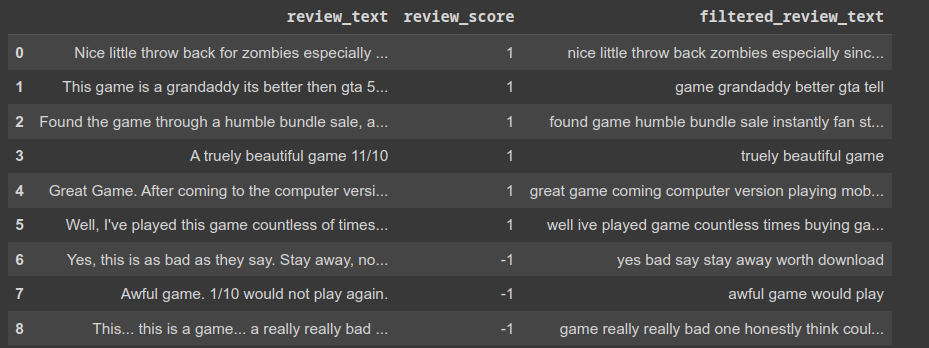
\includegraphics[scale=0.5]
{img/ex_data.png}
\centering
    
\end{frame}


\begin{frame}{Generating Filtered Review using Pre-trained Models}

\begin{table}[h]
\centering
\begin{tabular}{ll}
\toprule
\textbf{Model} & \textbf{Number of Parameters} \\
\midrule
gpt2 & 117M\\
gpt2-xl & 1558M\\
t5-base & 250M\\
t5-xl & 3000M\\
flan-t5-base & 250M\\
flan-t5-xl & 3000M \\
\bottomrule
\end{tabular}
\caption{Pre-tranied models}
\end{table}
\end{frame}

\begin{frame}{Pre-trained: Continue}
Prompt:
\begin{quote}
    "Keeps only sentimental words: \textit{review\_text}"
\end{quote}

\begin{itemize}
    \item Tokenization\\
    - Max\_length = 50\\
    \item Generate the most likely output\\
    - Max\_length = 25\\
    - early\_stopping\\
    - repetition\_penalty\\
    \item Decode
    
\end{itemize}


\end{frame}

\begin{frame}{Example}
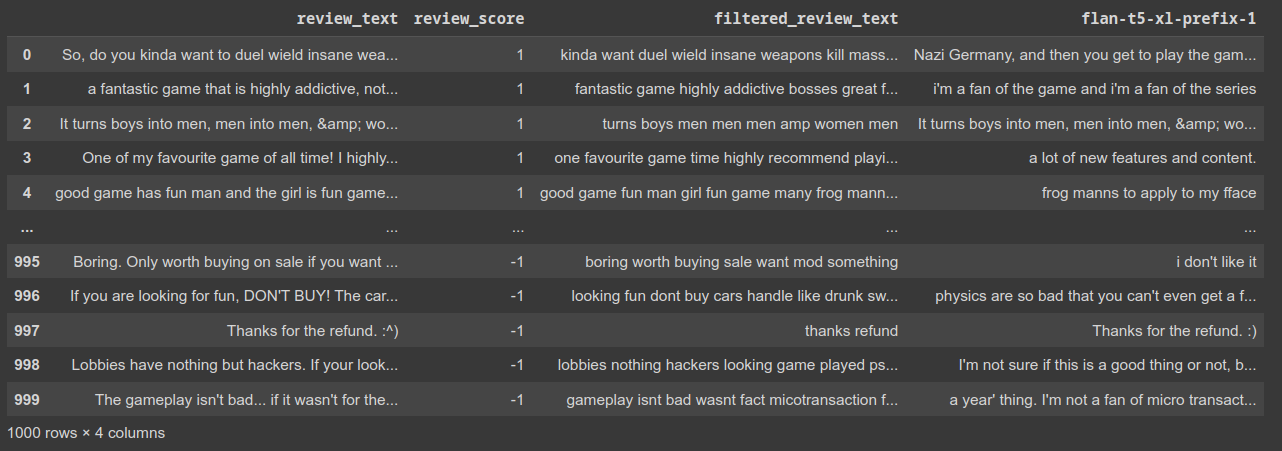
\includegraphics[scale=0.35]
{img/ex_pre_trained_data.png}
\centering
\end{frame}


\section{Validation}

\begin{frame}{Steam}
\begin{itemize}
\item Steam platform: largest digital distribution platform for video games
\end{itemize}

\includegraphics[width = \textwidth]
{img/1.png}
\centering
\end{frame}

\begin{frame}{Steam Review}
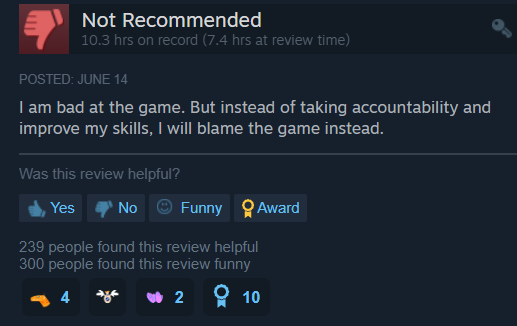
\includegraphics[width = \textwidth]
{img/2.png}
\centering
\end{frame}

\begin{frame}{Steam Review Dataset [1]}
\begin{itemize}
\item Approximately 6.8 million reviews.
\end{itemize}
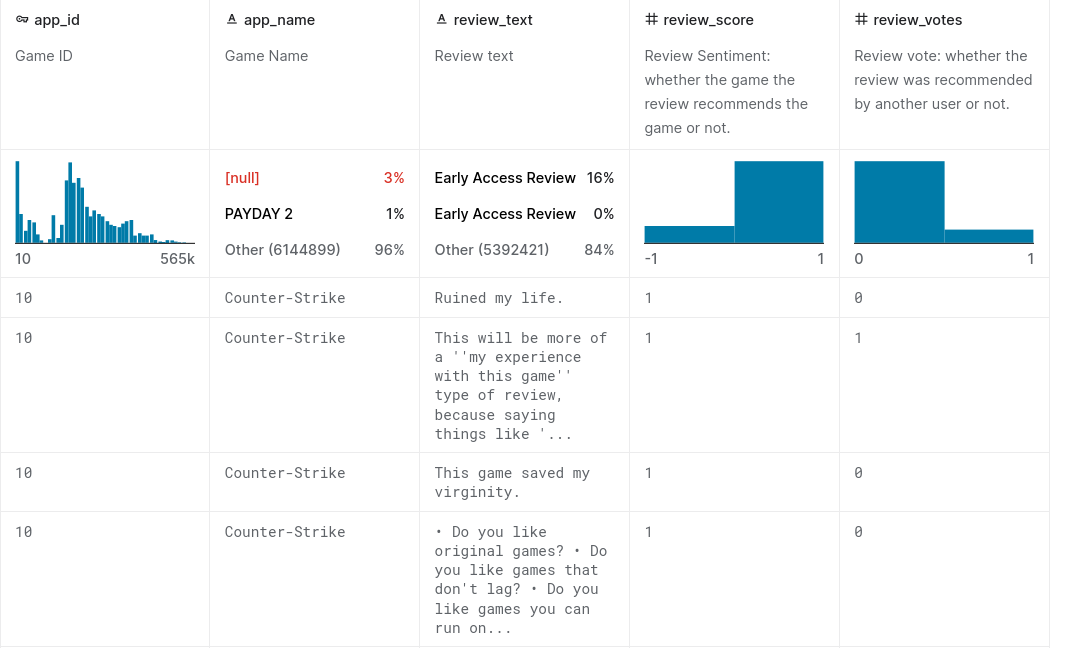
\includegraphics[width = \textwidth]
{img/fig_1.png}
\centering
\end{frame}
 

\begin{frame}{Text Vectorization: Bags of Words vs TFIDF}
\begin{itemize}
\item Importance weighting: Frequency, rarity, Importance
\item Reducing the impact of stopwords 
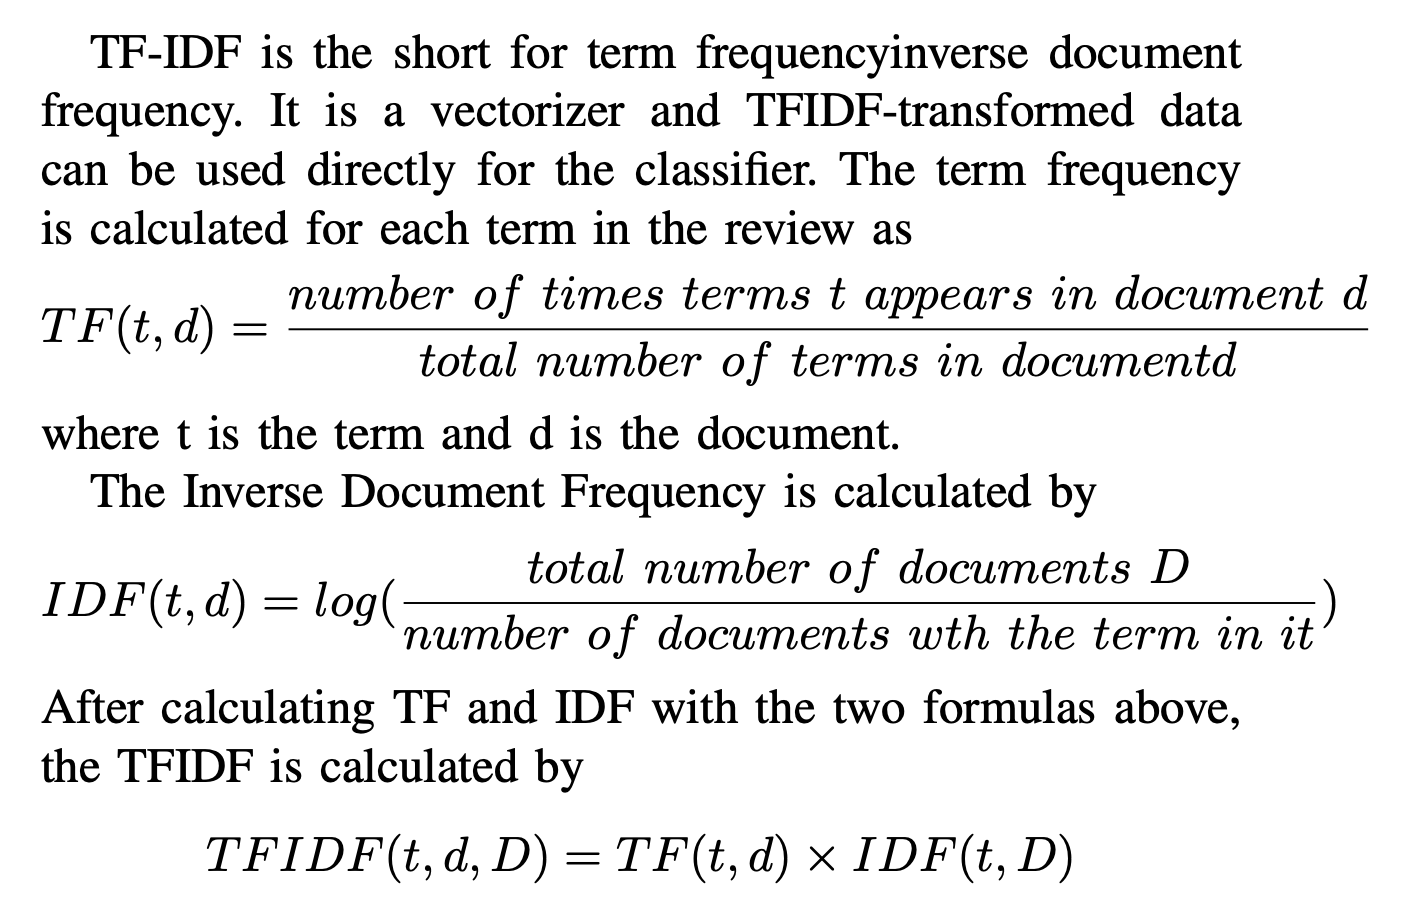
\includegraphics[width=\textwidth]{img/3.png}
\end{itemize}

\end{frame}

\begin{frame}{Multinomial Naive Bayes}
Given a document $d$ and a class label $c$, Bayes' theorem can be expressed as:

\begin{equation}
P(c|d) = \frac{P(d|c)P(c)}{P(d)}
\end{equation}

\begin{equation}
P(d|c)P(c) = P(w_1, w_2, \dots, w_n|c)P(c)
\end{equation}

where $w_1, w_2, \dots, w_n$ are the words in the document.

\end{frame}

\begin{frame}{Multinomial Naive Bayes continue}
\begin{equation}
P(w_1, w_2, \dots, w_n|c)P(c) = P(c)\prod_{i=1}^{n} P(w_i|c)
\end{equation}

To classify a document, we choose the class $c^*$ with the highest probability:

\begin{equation}
c^* = \arg\max_c P(c)\prod_{i=1}^{n} P(w_i|c)
\end{equation}
\end{frame}

\begin{frame}{Laplacian Smoothing}
    In practice, some words in the test data may not be present in the training data, leading to a zero probability for $P(w_i|c)$, which can cause issues in classification. To address this, Laplacian smoothing (also known as additive smoothing) is applied, which assigns a small non-zero probability to unseen words.

Given a word $w_i$ and a class $c$, the smoothed probability is calculated as:

\begin{equation}
P(w_i|c) = \frac{f_{w_i, c} + \alpha}{\sum_{w \in V} (f_{w, c} + \alpha)}
\end{equation}

where $f_{w_i, c}$ is the frequency of word $w_i$ in class $c$, $V$ is the vocabulary, and $\alpha$ is the smoothing parameter. A common choice for $\alpha$ is 1 (Laplace smoothing) or values between 0 and 1 (Lidstone smoothing).
\end{frame}
    

\begin{frame}{Linear SVM}
\textbf{Goal}: to find the optimal hyperplane that separates the data points of different classes with the maximum margin
\\
The decision function is a linear combination of the input features:

\begin{equation}
f(x) = w^T x + b
\end{equation}

where $w$ is the weight vector, $x$ is the input feature vector, and $b$ is the bias term.

The goal is to minimize the following objective function:

\begin{equation}
\frac{1}{2} |w|^2 + C \sum_{i=1}^{n} \xi_i
\end{equation}

subject to the some constrain function.
\end{frame}

\section{Results and Discussion}
\begin{frame}{Model Comparison MNB}

\begin{table}[h]
\centering
\begin{tabular}{llll}
\toprule
\textbf{Model} & \textbf{Mean Squared Error} & \textbf{Accuracy} & \textbf{F-1 Score} \\
\midrule
Baseline & 0.74 & 81.5 & 0.864 \\
gpt2 & 1.0 & 75.0 & 0.821 \\
gpt2-xl & 1.1 & 72.5 & 0.808 \\
t5-base & 1.3 & 67.5 & 0.758 \\
t5-xl & 1.08 & 73.0 & 0.80\\
flan-t5-base & 1.25 & 74.37 & 0.815 \\
flan-t5-xl & 1.14 & 71.356 & 0.78 \\
\bottomrule
\end{tabular}
\caption{Models performance on testing dataset evaluated using Naive Bayes with $a=0.1$ as smoothing parameter (fixed seed).}
\end{table}
\end{frame}

\begin{frame}{Model Comparison SVM}
\begin{table}[h]
\centering
\begin{tabular}{llll}
\toprule
\textbf{Model} & \textbf{Mean Squared Error} & \textbf{Accuracy} & \textbf{F-1 Score} \\
\midrule
Baseline & 0.7 & 82.5 & 0.865 \\
gpt2 & 1.18 & 70.5 & 0.784 \\
gpt2-xl & 1.2 & 70.0 & 0.781 \\
t5-base & 1.2 & 70.0 & 0.776 \\
t5-xl & 1.24 & 69.0 & 0.780\\
flan-t5-base & 0.96 & 75.87 & 0.821 \\
flan-t5-xl & 1.02 & 74.371 & 0.80 \\
\bottomrule
\end{tabular}
\caption{Models performance on testing dataset evaluated using SVM with $C=1$ as regularization parameters (fixed seed).}
\end{table}
\end{frame}

\begin{frame}{Discussion}
    \begin{enumerate}
    \item \textbf{Computational expense:} 


    \item \textbf{Time consumption:} Generating cleaned reviews using these models can be time-consuming.
    \begin{table}[h]
    \centering
    \begin{tabular}{ll}
    \toprule
    \textbf{Model} & \textbf{Generating time} \\
    \midrule
    gpt2 & 20m\\
    gpt2-xl & 1hr\\
    t5-base & 4m\\
    t5-xl & 25m\\
    flan-t5-base & 5m\\
    flan-t5-xl & 12m \\
    \bottomrule
    \end{tabular}
    \caption{Approximate generating time of 1000 reviews on a free Google Colab account}
    \end{table}

\end{enumerate}
\end{frame}

\begin{frame}{Disscussion: Continue}
        
    \begin{itemize}

    
    \item \textbf{Accessibility:} Many state-of-the-art models such as GPT-3/4 are not open-source but are accessible via paid APIs. This can be prohibitive for small businesses or individual developers who cannot afford the associated costs.
    
    \item \textbf{Prompt design:} It can be challenging to design optimal prompts when the model has not been fine-tuned, as the training details of the original model may not be available or clear. This lack of transparency can lead to inefficiencies and inaccuracies in the data cleaning process.
    
    \item \textbf{Knowledge requirement:} Fine-tuning these models requires extensive knowledge and understanding of their architecture and parameters. Finding optimal parameters can be challenging and may require a large amount of data and computational resources. This again can be expensive and beyond the means of many users.


    \end{itemize}
\end{frame}

\begin{frame}{Future Work}

\begin{itemize}
    \item \textbf{Fine-tuning FLAN-T5 for data cleaning:} We found that fine-tuning the FLAN-T5-base model on 300K reviews with a high-end GPU (40GB memory) and 70 compute units using Google Colab Pro took more than 9 hours. However, given the flexibility of the FLAN-T5 architecture in handling various NLP tasks, we believe it holds potential for being effectively fine-tuned to perform data cleaning tasks.
    
    \item \textbf{Exploring specialized deep learning models:} We plan to investigate more optimized deep learning models that are specifically designed for data cleaning tasks. This might help in enhancing the performance and reducing the computational overhead associated with current models.
    
    \item \textbf{Fine-tuning parameters:} There is scope for exploring different fine-tuning strategies, tokenizers, and model parameters to improve the efficacy of the pre-trained models in cleaning tasks.

\end{itemize}
\end{frame}

\begin{frame}{Future Work}
\begin{itemize}

        
    \item \textbf{Exploring optimal prompts:} Further work can be done to investigate and design optimal prompts for the pre-trained models to maximize their performance in data cleaning tasks.
\end{itemize}
\end{frame}

\begin{frame}{References}

\small

[1] Sobkowicz, A. (2017). Steam Reviews Dataset. Retrieved from \url{https://www.kaggle.com/datasets/andrewmvd/steam-reviews}

[2] Mukneam, P. (2023). sentiment\_steam. Retrieved from \url{https://github.com/pmukneam/sentiment_steam}

[3] Konduru, Y. J. (2021). Game Review Classifier. Retrieved from \url{https://yaswanth3277.github.io/Portfolio/gamereviewclassifier.html}

[4] Kumar, S. (2018). IMDB movie review polarity using Naive Bayes Classifier. Retrieved from \url{https://satyam-kumar.medium.com/imdb-movie-review-polarity-using-naive-bayes-classifier-9f92c13efa2d}

[5] Reddy, V. (2018). Sentiment Analysis using SVM. Retrieved from \url{https://medium.com/@vasista/sentiment-analysis-using-svm-338d418e3ff1}




\end{frame}

\begin{frame}{References: Continue}

[6] Narayanan, V., Aror, I.,\& Bhatia, A. (2013). Fast and accurate sentiment classification using an enhanced Naive Bayes model. Indian Institute of Technology.

[7] Zuo, Z. (2018). Sentiment Analysis of Steam Review Datasets using Naive Bayes and Decision Tree Classifier. Retrieved from \url{http://hdl.handle.net/2142/100126}

[8] Chu, X., Ilyas, I. F., Krishnan, S., \& Wang, J. (2016). Data Cleaning: Overview and Emerging Challenges. SIGMOD’16, June 26-July 01, 2016, San Francisco, CA, USA. DOI: \url{http://dx.doi.org/10.1145/2882903.2912574}



    
\end{frame}

\begin{frame}{References: Continue}


[9] Li, P., Rao, X., Blase, J., Zhang, Y., Chu, X., \& Zhang, C. (2021). CleanML: A Study for Evaluating the Impact of Data Cleaning on ML Classification Tasks. 2021 IEEE 37th International Conference on Data Engineering (ICDE), Chania, Greece. DOI: 10.1109/ICDE51399.2021.00009.

[10] Radford, A., Wu, J., Child, R., Luan, D., Amodei, D., Sutskever, I., \& others. (2019). Language models are unsupervised multitask learners. OpenAI blog, 1(8), 9.

[11] Raffel, C., Shazeer, N., Roberts, A., Lee, K., Narang, S., Matena, M., Zhou, Y., Li, W., \& Liu, P. J. (2020). Exploring the Limits of Transfer Learning with a Unified Text-to-Text Transformer. Journal of Machine Learning Research, 21(140), 1-67.

    
\end{frame}

\begin{frame}{References: Continue}


[12] Chung, H. W., Hou, L., Longpre, S., Zoph, B., Tay, Y., Fedus, W., Li, E., Wang, X., Dehghani, M., Brahma, S., \& others. (2022). Scaling Instruction-Finetuned Language Models. arXiv. \url{https://arxiv.org/abs/2210.11416}

[13] Mukneam, P. (2023). sentiment-deep-cleaning. Retrieved from \url{https://github.com/pmukneam/sentiment-deep-cleaning}
    
\end{frame}


\end{document}



